\documentclass[11pt]{article}
%\usepackage[14pt]{extsizes} % для того чтобы задать нестандартный 14-ый размер шрифта
%\usepackage[utf8]{inputenc}
\usepackage{mathtext}
\usepackage[english, russian]{babel}
\usepackage{amsmath}
\usepackage{amsfonts}
\usepackage{float}
\usepackage[margin=0.8in]{geometry}
\usepackage{multirow}
\usepackage{graphicx}
\usepackage[utf8x]{inputenc} % указать кодировку русского текста
\usepackage{fancyhdr}
\usepackage{indentfirst} % отступ в первой строке абзаца
\usepackage{wrapfig}
\usepackage{placeins}
\usepackage{wrapfig}
\usepackage{caption}
\usepackage{amssymb}
\usepackage{mathtools}
\usepackage[thinc]{esdiff}
\usepackage{cmap}
\usepackage[table,xcdraw]{xcolor}

\pagestyle{fancy}
\begin{document}
\begin{titlepage}
\begin{center}
%\vspace*{1cm}
\large{\small ФЕДЕРАЛЬНОЕ ГОСУДАРСТВЕННОЕ АВТОНОМНОЕ ОБРАЗОВАТЕЛЬНОЕ\\ УЧРЕЖДЕНИЕ ВЫСШЕГО ОБРАЗОВАНИЯ\\ МОСКОВСКИЙ ФИЗИКО-ТЕХНИЧЕСКИЙ ИНСТИТУТ\\ (НАЦИОНАЛЬНЫЙ ИССЛЕДОВАТЕЛЬСКИЙ УНИВЕРСИТЕТ)\\ ФИЗТЕХ-ШКОЛА РАДИОТЕХНИКИ И КОМПЬЮТЕРНЫХ ТЕХНОЛОГИЙ}
\vfill
\line(1,0){430}\\[1mm]
\huge{Лабораторная работа 4.5.3}\\
\huge\textbf{Сканирующий интерферометр}\\
\line(1,0){430}\\[1mm]
\vfill
\begin{flushright}
\normalsize{Устюжанина Мария}\\
\normalsize{\textbf{Группа Б01-107}}\\
\end{flushright}
\end{center}
\end{titlepage}
\fancyhead[L] {Работа 4.5.3}

\par \textbf{Цель работы:} Знакомство с устройством и работой газового лазера непрерывного действия, со спектральными характеристиками лазерного излучения, а также с устройством и принципом действия сканирующего интерферометра Фабри—Перо.


\par \textbf{В работе используются:} 
\(He-Ne\)-лазер с блоком питания; сканирующий интерферометр Фабри—Перо; поляроид; пластинка \(\lambda / 4\); линза;
фотодиод; электронный осциллограф.


\section{Установка}

\begin{figure}[H]
  \centering
  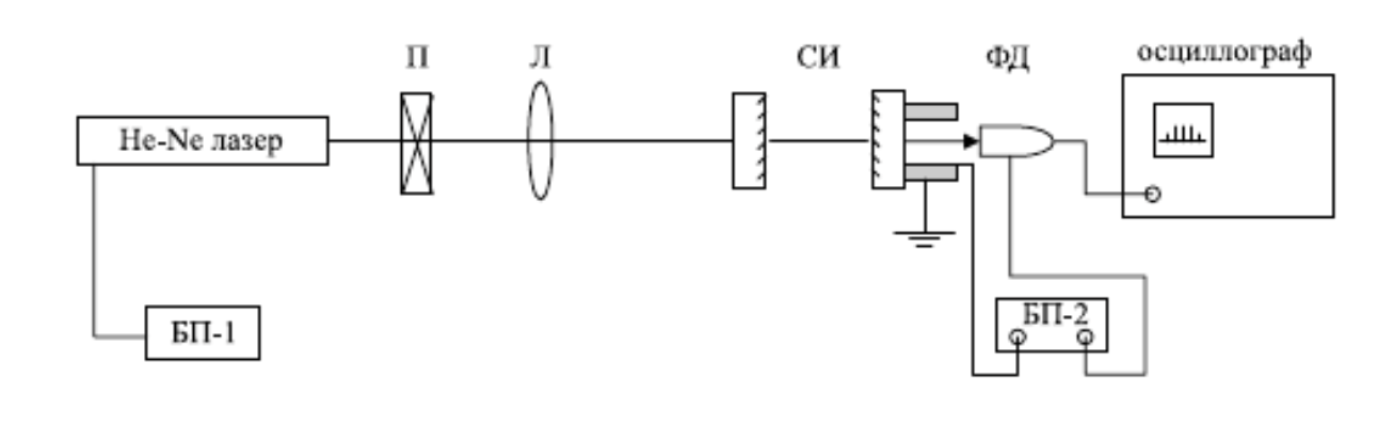
\includegraphics[width=\textwidth]{1.png}
  \caption{Схема экспериментальной установки}
  \label{fig:device}
\end{figure}

\begin{figure}[H]
  \centering
  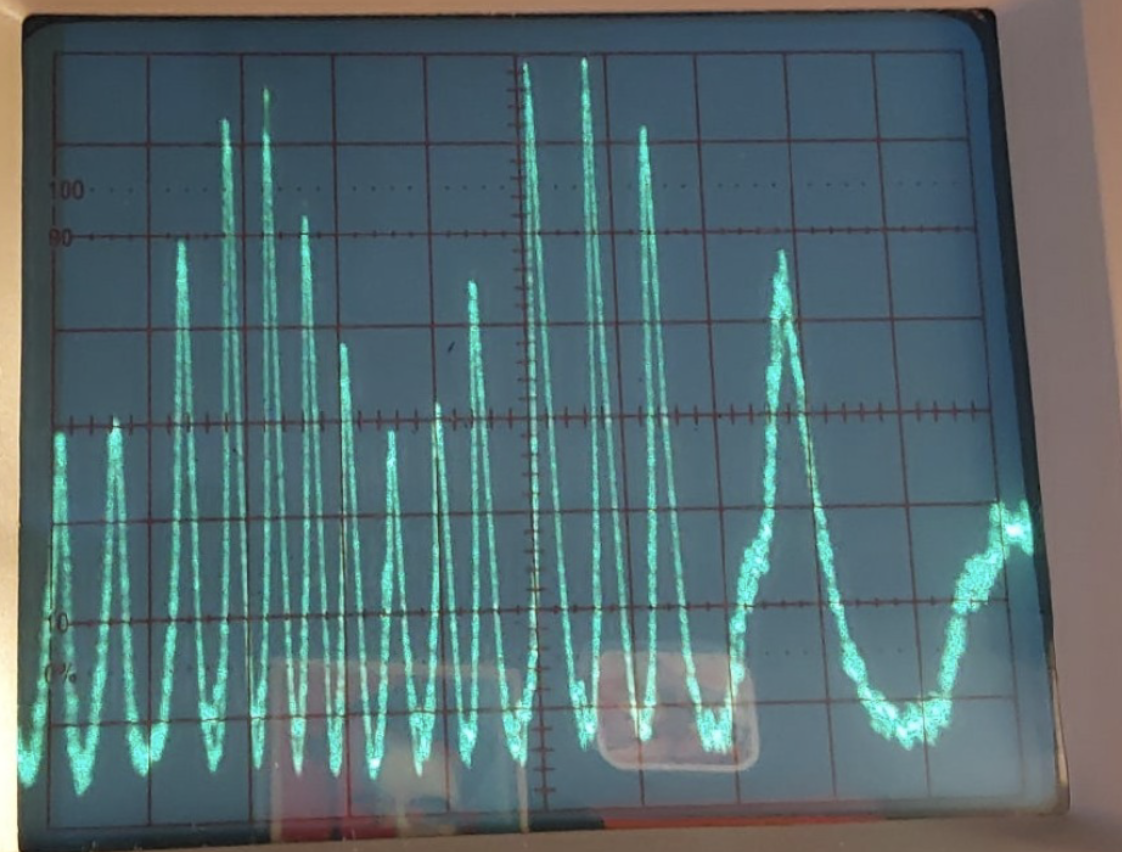
\includegraphics[width=\textwidth]{2.png}
  \caption{Картина мод на осциллографе}
  \label{fig:modes}
\end{figure}



\section{Ход работы:}

\begin{enumerate}

  \item Вычислим межмодовое расстояние резонатора в единицах \(\nu\) и \(\lambda\). Учитывая, что длина лазера \(L = 65\:см\)
и \(\lambda = 632.8\cdot 10^{-9}\:м \)

\[ \Delta\nu = \nu_{m+1} - \nu_m = \frac{c}{2L} \simeq 2.3\cdot10^8\; Гц\]
\[ \Delta\lambda = \lambda_{m+1} - \lambda_m = \frac{\lambda^2}{2L} = 0.3\cdot 10^{-12}\:м \]

  \item По картине на осцилографе определим число промежутков между модами внутри одного доплеровского контура:
\[ N = 6 \pm 1 \]

 \item Найдем видимую ширину спектральной линии неона:
\[ \Delta\lambda_{Ne} = \frac{m\cdot\Delta\lambda }{2} = \left( 0.9 \pm 0.15  \right)\cdot 10^{-12}\:м \]  

  \item Учитывая, что ширина спектральной линии обусловлена эффектом Доплера и что видимая ширина линии неона порядка полуширины доплеровского контура 
\(\left[\Delta\lambda\left(Ne\right) \simeq \Delta\lambda_D\right]\), найдем среднюю скорость атомов неона вдоль оси лазера:
\[ v_x \simeq \frac{\Delta\lambda_D}{\lambda}\cdot c \simeq \left( 426 \pm 71 \right)\; м/с \]
А также значение газокинетической температуры (\( m = 33.5\cdot 10^{-27}\: кг\)):
\[ \frac{mv_x^2}{2} = \frac{kT}{2} \Rightarrow T = \frac{mv_x^2}{k} = 440 \pm 145 K  \]

  \itemНайдем дисперсионную область сканирующего интерферометра:
\[ \Delta\lambda_{SI} = \frac{\lambda}{m} = \frac{\lambda^2}{2l} = 
\frac{\left(632.8\cdot 10^{-9}\right)^2}{2 \cdot 0.09} \simeq 2.2\cdot 10^{-12}\;м  \]
она получилась в 2 раза больше, чем \(\Delta\lambda_{Ne}\)

  \itemСравним значения ширины отдельной моды на полувысоте с межмодовым расстоянием: 
\[ n = 3 \pm 0.5 \]

\itemНайдем разрешение \(\delta\lambda\) сканирующего интерферометра:
\[ \delta\lambda = \frac{\Delta\lambda}{n} = \left(0.1 \pm 0.016\right)\cdot 10^{-12}\;м \]
\itemОценим разрешающую способность:
\[ R = \frac{\lambda}{\delta\lambda} = = \left(6.328 \pm 1.012 \right)\cdot 10^6 \]
\itemРассчистаем коэффициент отражения  зеркал интерферометра:
\[ R = \frac{2\pi l}{\lambda(1-r)} \Rightarrow r = 1 - \frac{2\pi l}{\lambda R} = 0.86 \pm 0.02  \]
\end{enumerate}

\section{Выводы}

  \par Мы в ходе работы познакомились со сканирующим интерферометром Фабри—Перо.
  \medskip
  \par Нашли видимую ширину спектральной линии неона:
  \[ \Delta\lambda_{Ne} = \left( 0.9 \pm 0.15  \right)\cdot 10^{-12}\: м \]
  \par  Оценили среднюю скорость атомов неона вдоль оси лазера:
  \[ v_x = \left( 426 \pm 71 \right)\; м/с \]
  \par  Посчитали газоеинтеическую температуру атомов неона:
  \[ T = \left(440 \pm 145 \right)\;K \]
  \par  Нашли разрешение интерферометра Фабри-Перо:
  \[ \delta\lambda = \left(0.10 \pm 0.02\right)\cdot 10^{-12}\;м \]
  \par  Оценили разрешающую способность интерферометра:
  \[ R = \left(6 \pm 1 \right)\cdot 10^6 \]
  \par  Посмитали коэффициент отражения зеркал интерферометра:
  \[ r = \left(0.86 \pm 0.02 \right) \]



\end{document}